\section{Projeto de energia}

O grupo de engenharia de energia é responsável pela análise e escolha da fonte energética do projeto, pelo estudo do tempo de duração da carga desta fonte, bem como o dimensionamento do sistema fotovoltaico off-grid a ser instalado.

\subsection{Motor}
Neste projeto será utilizado o motor elétrico, que é uma máquina de construção simples,e que possui uma grande versatilidade de adaptação às cargas dos mais diversos tipos e potências.

Entre os tipos de motores estão os de corrente alternada e os de corrente contínua. Foi escolhido o de corrente contínua, pois apesar do seu custo mais elevado, ele funciona com velocidade ajustável entre amplos limites e se prestam a controles de grande flexibilidade e precisão.

\subsubsection{Dimensionamento do Motor}

Para a definição de capacidade de dosagem do sistema de dosagem, utilizou-se a equação abaixo:

\begin{center}
$Q=4,71.10^{-5}.(D^{2}-d^{2}).p.n$
\end{center}

Onde:

$Q = capacidade, m^3/h;$

$D = diâmetro da rosca tubular, cm;$

$d = diâmetro interno do helicóide, cm;$

$p = passo do helicóide, cm e$

$n = rotação, rpm.$

\begin{center}
$Q=4,71.10^{-5}.(5^{2}-1,5^{2}).4,4.28$
\end{center}

Cálculo da potência requerida:

\begin{center}
$Pt = 2,22.10^{-4}.(Q.\mu.L.\emptyset)$
\end{center}

Onde:

$Pt = potência requerida pelo transportador, cv;$

$Q = capacidade, m^3/h;$

$\mu = massa específica do material, kg/m^3;$

$L = comprimento total do transportador, m e$

$\emptyset = fator de potência, adimensional.$


\begin{center}
$Pt = 2,22.10^{-4}.(0,0022.234,7.1.0,4)$

$Pt = 0,0004585*2$

$Pt = 0,0009701 CV$

\end{center}

A potência é multiplicada por 2, pois quando seu valor é menor que 1,0 , deve-se aplicar o fator de correção no valor de 2.\\

Cálculo do torque:\\

$T=9550.\frac{Pt}{n}$\\

Onde:

$T = torque, N,m;$

$Pt = potência requerida pelo transportador, kW;$

Logo, o tem-se um torque requerido de $T=0,023N.m$

\subsubsection{Motor DC}

Para atender os requistos do projeto, a princípio será utilizado um motor da marca Bosh, modelo F006 B20 321, que já está disponível para a equipe, e que será testado na rosca helicoidal posteriormente.

\begin{figure}[H]
 \centering
   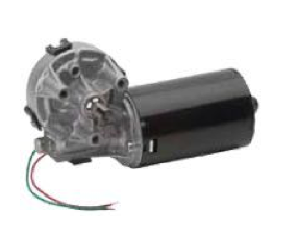
\includegraphics[keepaspectratio=true,scale=0.8]{figuras/motor2.eps}
 \caption{Motor}
 \label{motor2}
\end{figure}

\subsection{Sistema de Alimentação de Energia}
O sistema de alimentação de energia será por meio de placa fotovoltaica, visto que o alimentador de peixes ficará no meio do lago, e não será possível fazer recarga de bateria. O sistema de geração é composto por:

\begin{itemize}
    \item Painel Solar Fotovoltaico
    \item Bateria
    \item Controlador de Carga
    \item Cabos para conexão do equipamento
    \item Suporte para o painel fotovoltaico

\end{itemize}

\subsubsection{Painel Solar Fotovoltaico}
A grande vantagem da utilização da energia solar no projeto, é que esta é uma fonte renovável e sustentável. Além disso, o sistema tem um baixo custo de manutenção e longa vida útil. Quando houver energia excedente, a energia será armazenada na bateria estacionária.
Como atividade futura, será dimensionado o painel a ser utilizado na estrutura do alimentador de peixes, onde o mesmo para ser viável, não poderá ter dimensões maiores que a estrutura.

\subsubsection{Bateria}

Será necessária a utilização de uma bateria como de alimentação de motores e componentes eletrônicos do projeto, devido à incapacidade na utilização de energia elétrica e na praticidade ao utilizar a energia solar já disponível no local.

A bateria é utilizada nos sistemas fotovoltaicos para armazenar energia excedente produzida pelos painéis, para ser utilizada durante a noite ou em dias nublados ou com baixa insolação. As mais utilizadas em sistemas de energia renovável são as do tipo estacionárias ou de ciclo profundo, pois suportam grandes descargas que uma bateria comum não suportaria.

\begin{figure}[H]
 \centering
   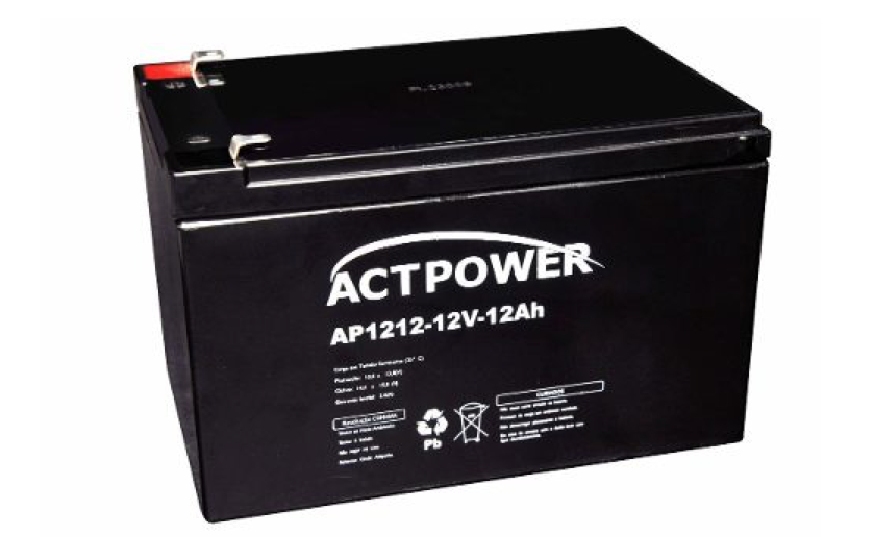
\includegraphics[keepaspectratio=true,scale=0.8]{figuras/motor1.eps}
 \caption{bateria estacionaria}
 \label{motor1}
\end{figure}

\begin{itemize}
\item{Dimensionamento da Bateria}
\end{itemize}

Conforme a potência total requerida pelo sistema (motor + componentes eletrônicos), 19 W + 2 W, calculou-se a corrente necessária.

Cálculo da corrente:

\begin{center}$P_{motor}=19\,W$


$P_{eletronica}=2\,W$


$P_{total}=P_{motor}+P_{eletronica}=21\,W$


$i=\frac{P}{V}$


$i(motor)=\frac{19}{12} = 1,58\,A$


$i(eletronica)=\frac{2}{12} = 0,166\,A$

\end{center}


Considerando a autonomia de 2h para o motor, e 24h para os componentes eletrônicos, calculou-se a capacidade da bateria.

\begin{center}
$Capacidade=(1,58\times2h).(0,166\times24h)=7,144\,Ah$

\end{center}

Assim, a capacidade da bateria é 7,144 Ah, porém não é recomendado a descarga total, devido reduzir a vida útil da bateria. Considerando uma descarga de 75\%, calculou-se a capacidade para bateria.

Cálculo Capacidade da Bateria:

\begin{center}
$Ah=\frac{7,144\,Ah}{0,75}$


$Ah=9,525$
\end{center}

\subsubsection{Controlador de Carga}
Será utilizado um controlador de carga acoplado aos paineis
fotovoltaicos e a bateria para realizar o controle do sistema.O controlador é responsável pela duração da vida útil dos bancos de baterias protegendo-o contra sobretensões e descargas excessivas. Assim, é de fundamental importância a utilização de um controlador de cargas. Esses controladores se localizam entre painéis fotovoltaicos e baterias onde controla-se a tensão de entrada já que as baterias não suportam grande flutuação de energia. Sendo assim, permite que as baterias sejam carregadas de melhor forma informando o estado de carga da bateria (SERRÃO, 2010).

\subsubsection{Custos do projeto de energia}

\begin{table}[H]
\centering
\caption{Tabela de custo do projeto de energia}
\label{custo_energia}
\begin{tabular}{|l|l|}
\hline
MATERIAL             & VALOR      \\ \hline
Placa Fotovoltaica   & R\$ 150,00 \\ \hline
Controlador de Carga & R\$ 150,00 \\ \hline
Bateria estacionária & R\$ 200,00 \\ \hline
Suporte e Cabos      & R\$ 50,00  \\ \hline
Motor                & R\$ 150,00 \\ \hline
Total                & R\$ 700,00 \\ \hline
\end{tabular}
\end{table}
